\documentclass[11pt]{standalone}

\usepackage{ifthen}
\usepackage{tikz} 
\usetikzlibrary{shapes.misc}
\usetikzlibrary{arrows,arrows.meta}
\usetikzlibrary{calc,intersections, patterns, math}

\definecolor{pfeil}{RGB}{168,167,167}
\definecolor{petrol}{RGB}{0, 118, 136}
\definecolor{darkgoldenrod}{RGB}{184, 134, 11}
\colorlet{petrol-lighter}{petrol!40}
\colorlet{darkgoldenrod-lighter}{darkgoldenrod!40}

\begin{document}

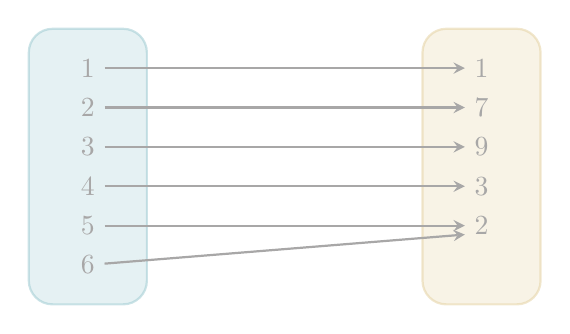
\begin{tikzpicture}[pfeil]

    \draw[thick, fill=petrol!20, draw=petrol-lighter, rounded corners=2ex, opacity=0.5] (0,0) rectangle ++ (1.5,3.5);
    \draw[thick, fill=darkgoldenrod!20, draw=darkgoldenrod-lighter, rounded corners=2ex, opacity=0.5] (5,0) rectangle ++ (1.5,3.5);

    \foreach \x in {1, ..., 6}{
            \node (D\x) at (0.75,3.5-0.5*\x) {\x};
        }

    \foreach \x/\y in {1/1,2/7,3/9,4/3,5/2}{
            \node (Z\x) at (5.75,3.5-0.5*\x) {\y};
        }


    \foreach \x in {1,...,5}
				\draw[thick,-stealth] (D\x) -- (Z\x);

    \draw[thick,-stealth,] (D6) -- (Z5.base west);

\end{tikzpicture}

\end{document}
